\PassOptionsToPackage{svgnames,dvipsnames,svgnames}{xcolor}
\documentclass[10pt]{article}
\usepackage{microtype} 
% \usepackage{times}
\usepackage[T1]{fontenc}
\usepackage{soul}
\usepackage{mathpazo}
\usepackage[hmargin=1in,vmargin=1in]{geometry}
\usepackage{todonotes}
\usepackage{listings}
\lstset{tabsize=2, 
basicstyle=\ttfamily\fontsize{9pt}{1em}\selectfont, 
commentstyle=\itshape\ttfamily\color{gray}, 
stringstyle=\ttfamily\color{red},
mathescape=false,escapechar=\#,
numbers=left, numberstyle=\scriptsize\color{gray}\ttfamily, language=ML,moredelim=[il][\sffamily]{?},showspaces=false,showstringspaces=false,xleftmargin=15pt, morekeywords=[1]{tyfam,opfam,let,fn,val,def,casetype,objtype,metadata,of,*,datatype,new,toast,syntax,module,where,import,for,ana,syn,opcon,tycon,metasignature,metamodule,metasig,metamod,static,at,tycase,mod,macro,match,float,pattern,in,patterns,expressions,implicit,forall,rectype,fold,unfold,inj,by,spliced},deletekeywords={double},classoffset=0,belowskip=\smallskipamount,
moredelim=**[is][\color{red}]{SSTR}{ESTR},
moredelim=**[is][\color{Green}]{SHTML}{EHTML},
moredelim=**[is][\color{purple}]{SCSS}{ECSS},
moredelim=**[is][\color{brown}]{SSQL}{ESQL},
moredelim=**[is][\color{orange}]{SCOLOR}{ECOLOR},
moredelim=**[is][\color{magenta}]{SPCT}{EPCT}, 
moredelim=**[is][\color{gray}]{SNAT}{ENAT}, 
moredelim=**[is][\color{Green}]{SURL}{EURL},
moredelim=**[is][\color{SeaGreen}]{SQT}{EQT},
moredelim=**[is][\color{Periwinkle}]{SGRM}{EGRM},
moredelim=**[is][\color{YellowGreen}]{SID}{EID},
moredelim=**[is][\color{Sepia}]{SUS}{EUS},
deletestring=[d]{"},
}
\lstloadlanguages{Java,VBScript,XML,HTML,ML}
\let\li\lstinline

\usepackage{newtxtt}
\usepackage{enumitem}

\newcommand{\HazelEnv}{Hazel}

\begin{document}
\section*{Research Statement}
My research aims to bring to life a new generation of highly \emph{adaptable} and \emph{intelligent} programming systems.

By \emph{adaptable programming system}, I mean one that allows the libraries that the programmer has imported to install new syntactic, semantic and edit-time features. Adaptability has become critical as programming has pervaded society, because language and tool designers can no longer hope to satisfyingly accomodate every problem domain. A major difficulty lies in ensuring that these library-specific features do not interfere with one another, nor weaken the type and binding discipline of the language (because a language with a strong type and binding discipline is, I am thoroughly convinced, necessary for programming ``in the large''.)% I have taken a leading role in the community of researchers aiming to address this problem. % At their core, the languages of the future will be based on the foundational principles of type theory.

By \emph{intelligent programming system}, I mean one that combines a semantic understanding of the program being written with statistics gathered from other programs to generate code suggestions, and more generally \emph{action suggestions}, for the programmer throughout the programming process. There are many careers worth of difficulties that await confrontation here. My interest is in developing principled solutions to foundational problems, including (1) the problem of extracting meaning from programs that are not complete; (2) the problem of reasoning about edit actions as formal structures; and (3) the problem of combining semantic and statistical approaches to suggestion generation.

Solutions to these problems promise to have a broad impact on language and tool design. I am particularly interested in designing better languages and tools for (1) scientists, broadly construed; and (2) individuals with severely limited mobility and other physical disabilities. I have a distinctive perspective on these topics because as an undergraduate and, from 2008 to 2010, as a PhD student in neuroscience, (1) I developed computational models of neurobiological circuits in the sensorimotor system; and (2) I studied, and built, neural prosthetics (a.k.a. brain-computer interfaces.)

% My approach is to start from the first principles of type theory, probability theory and information theory. I then apply disciplined qualitative and empirical methods as I scale up, validate and iterate on my designs.


\subsection*{Previous and Ongoing Research}
\subsubsection*{Adaptable Programming Systems}

Over the course of my graduate studies, I have developed several mechanisms that allow libraries to install new language and editor features in a manner that protects clients from conflicts and semantic confusion.

My PhD thesis focuses on mechanisms that allow libraries to install type-specific syntactic sugar. For example, consider a web programming library that defines a type, \li{Element}, for HTML elements. Using the mechanisms I have developed, the library provider can equip this type with HTML syntax. Clients of this library can use this syntax wherever a value of type \li{Element} is expected, e.g.
\begin{lstlisting}[numbers=none]
val body : Element = `SURL<p>Hello, {[EURLjoin ' ' [first, last]SURL]}</p>EURL`
\end{lstlisting}
Uniquely, syntactic conflicts are impossible by construction, because the outer delimiters (here, backticks) are fixed, and control over parsing the body (between backticks) is delegated in a deterministic, type-directed manner. Moreover, the mechanism comes equipped with a principle of \emph{syntactic abstraction}, meaning that library clients can reason about types and binding without examining the expansions of newly installed syntactic forms like these. The core mechanism was formally introduced in a paper at \textbf{ECOOP 2014}, which was awarded a \textbf{Distinguished Paper Award}. It was  also covered widely by the popular programming press, and our implementation now has over 400 stars on GitHub.
% A subsequent refinement of this core mechanism, in collaboration with an undergraduate summer student, was described in a short paper at \textbf{SAC 2015}. 
My dissertation formalizes variants of this mechanism that interact with advanced language features, including pattern matching, parameterized types and ML-style modules. An account of this subsequent research was awarded \textbf{2nd place at the ICFP 2015 Student Research Competition}, and a capstone journal publication based on these results is in preparation for submission in the spring.

I have also developed a mechanism that gives library providers the ability to install new \emph{semantic fragments}. Fragment definitions are delegated control over typechecking and translation (to a fixed target language) in a type-directed manner. In our paper at \textbf{GPCE 2016}, we argue that this design is compositionally well-behaved and expressive, with examples of
fragments that express the static and dynamic semantics of
1) functional primitives (e.g. records and labeled sums, with support for nested pattern
matching \emph{a la} ML); 2) a variation on JavaScript's prototypal
object system; 3) typed foreign interfaces to Python and
OpenCL; and 4) a system of constrained string types useful for verifying that strings have been securely sanitized as intended. This last fragment, developed in collaboration with an undergraduate research student, was described formally in a paper at the \textbf{PSP 2014} workshop, where it was awarded the \textbf{Best Paper Award}.

Finally, I have developed a mechanism that allows library providers to install type-specific {graphical user interfaces} for code generation into the client's program editor. Clients are offered access to these interfaces via the standard code completion menu based on the type of expression being entered at the cursor. In a paper published at \textbf{ICSE 2012}, we describe this system and our human-centered design process. In particular, we began by gathering feedback on our initial mockups from over 450 professional software developers via an online survey. This resulted in a ranked collection of design criteria that guided our final design. We validated our final design with a controlled pilot study.

\subsubsection*{Intelligent Programming Systems}
Programming language definitions assign meaning to \emph{complete} programs. 
Programmers, however, spend a substantial amount of time interacting with \emph{incomplete} programs using tools like program editors and live programming environments (which interleave editing and evaluation.) If these systems are to intelligently suggest edit actions to the programmer, they need (1) to be able to extract meaning from incomplete programs; (2) to have access to a meaningful language of structured edit actions; and (3) to incorporate a statistical model of incomplete programs, so that the suggestions can be ranked by likelihood.

I have led the development of a foundational calculus called Hazelnut that addresses the first two of these problems. This calculus, described in a paper appearing at \textbf{POPL 2017}, assigns static meaning to programs that contain \emph{holes} and \emph{type inconsistencies}. Interestingly and encouragingly, the machinery for type holes coincides with that developed in the study of gradual type systems. The paper then develops an \emph{action semantics} that assigns meaning to structured edit actions and maintains a powerful invariant: that every well-defined action leaves the program statically meaningful, according to the aforementioned static semantics. We have mechanized the metatheory of Hazelnut using the Agda proof assistant. We also have a web-based implementation of a simple {structure editor} based on this calculus. It is written in OCaml using functional reactive programming techniques, and compiled using \li{js_of_ocaml}.

With respect to the problem of developing a statistical model of programs, I have led two projects of note. 
First, during my years as a neuroscientist, I developed a principled information theoretic framework for designing \emph{neural prosthetics}, i.e. systems used by paralyzed and locked-in individuals to communicate commands (i.e. simple programs) to various devices -- we used speech synthesizers, motorized wheelchairs, and (because everyone deserves to have some fun) prop airplanes. This framework, which was published in a special issue of the {International Journal of Human-Computer Interaction} (\textbf{IJHCI 2010}), relies on a statistical understanding of both the communication channel (in our system, an EEG headset) and  the language of commands (which has, thusfar, been very simple.)

The second project, which began as a course project for a Machine Learning course and remains ongoing as of this writing, involves developing a principled statistical model of well-typed expressions that takes into account the form, the type and the context around the expression being evaluated for insertion. In our preliminary investigations, our simple model already keeps pace with or outperforms state of the art models that use a fundamentally \emph{ad hoc} tokenized representation of programs. % These early results were awarded 3rd place at the SPLASH 2014 Student Research Competition.



\subsubsection*{Computational Neuroscience and Neuroinformatics}

I received bachelors degrees in Computer Science and Molecular \& Cellular Biology from UIUC, and entered graduate school at CMU in the Neural Computation PhD program. There, I worked in collaboration with an experimental neurophysiologist on a computational model of a neurobiological circuit in the portion of the rat somatosensory cortex responsible for whisker sensations. This research was published in the \textbf{Journal of Neuroscience (2012)}. I then became interested in the problem of systematically validating scientific models like these against empirical data on an ongoing basis. Our solution, which combines testing techniques, statistical techniques and modularity techniques, was described in a short paper at \textbf{ICSE 2014} (NIER track, 18\% acceptance rate.) My collaborator, Rick Gerkin (now faculty at ASU), continues to push forward on this project, funded by an R01 grant from the National Institutes of Health. I contributed to the writing of this grant and continue to have an advisory role in the project. My transfer to the Computer Science program to work primarily on programming languages and environments was precipitated by my experiences as a neuroscientist --- I became convinced that we need better tools before we will be able to develop a systematic understanding of systems as complex as a brain!



\subsection*{Future Research Directions}
\begin{figure}
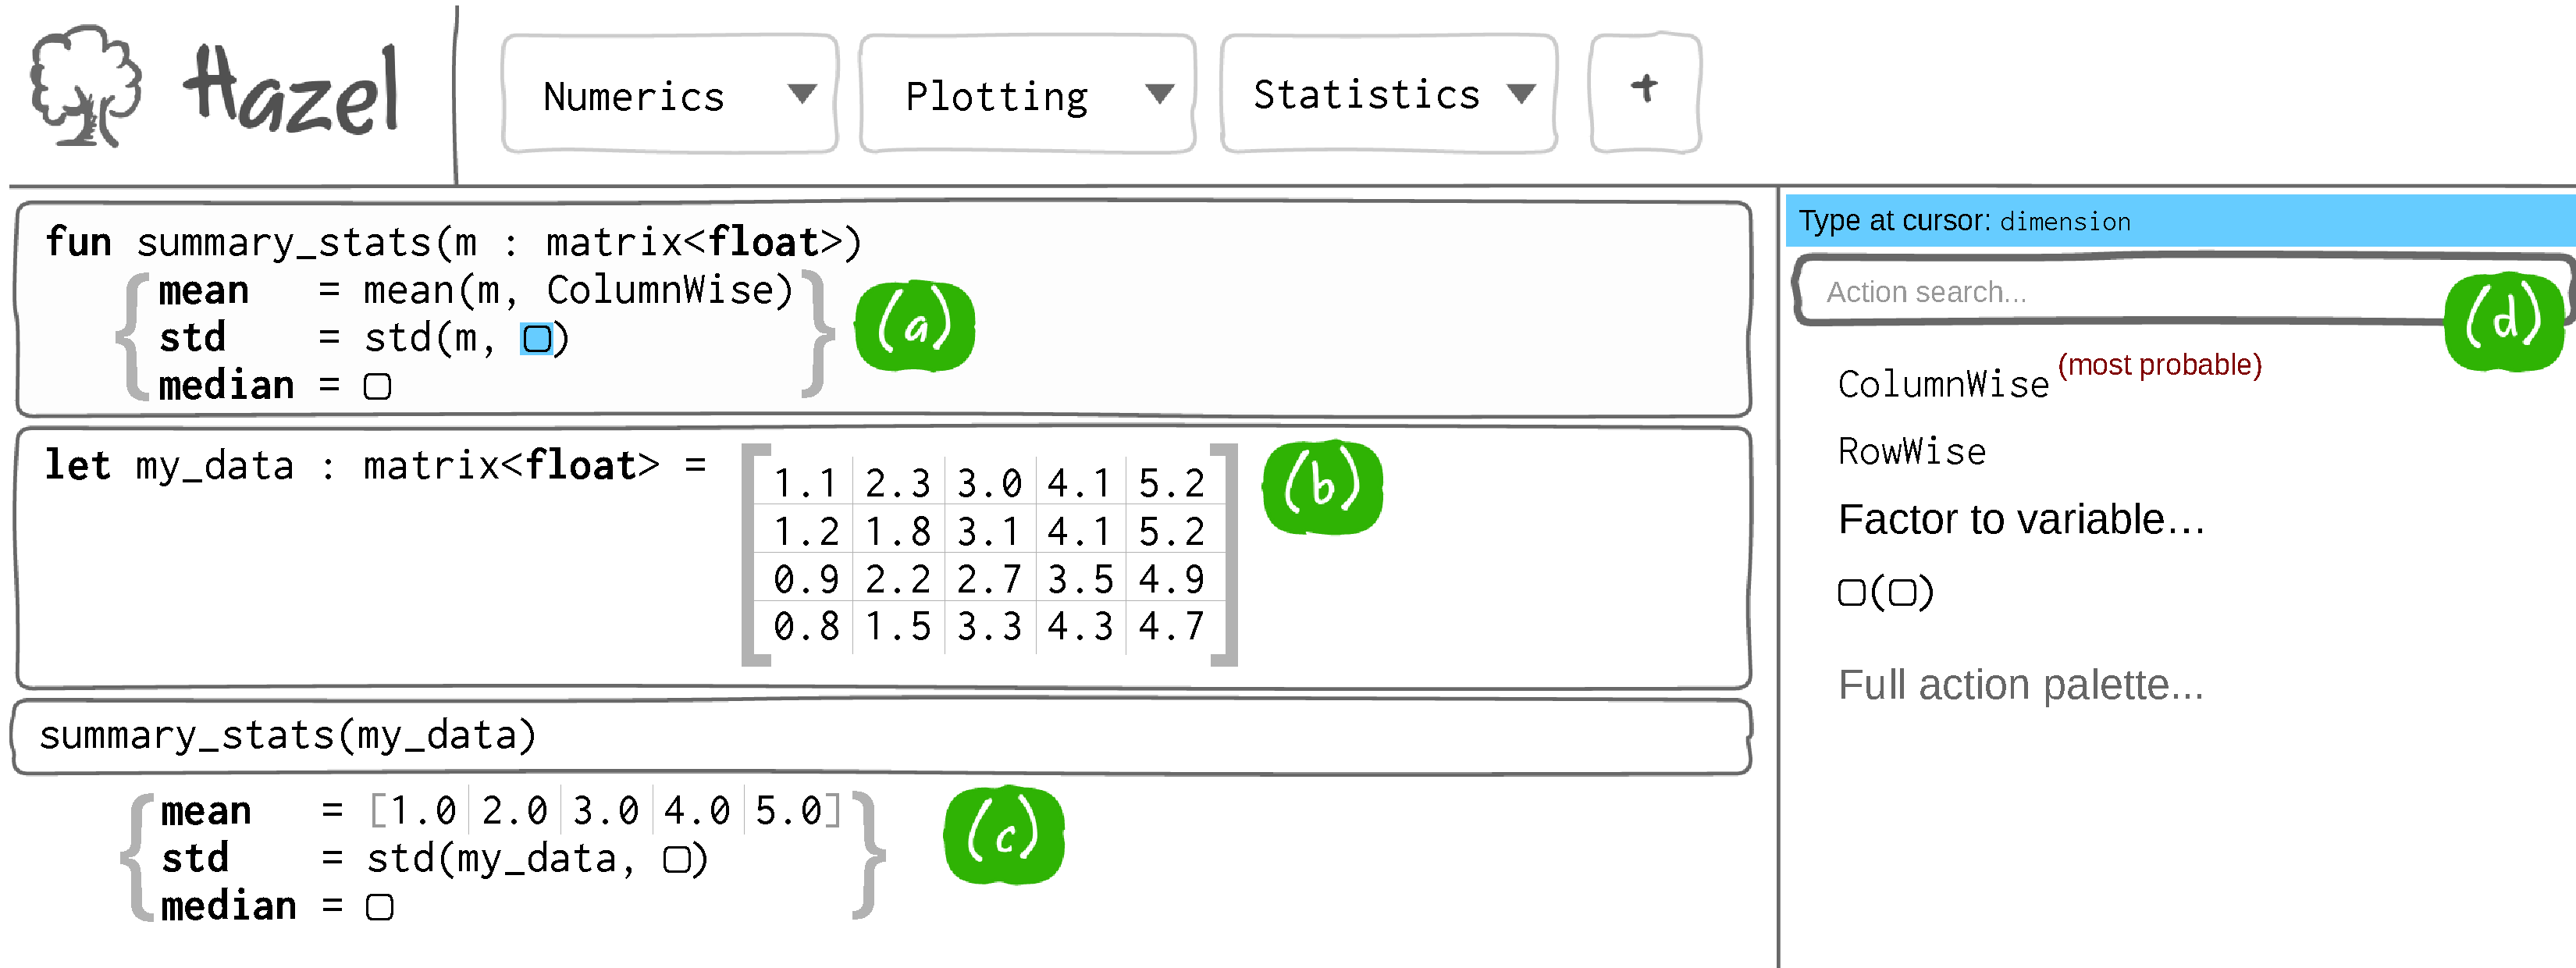
\includegraphics[width=\textwidth]{mockup-1}
\vspace{-3ex}
\caption{A mockup of Hazel.}
\label{fig:hazel-mockup}
\vspace{-2ex}
\end{figure}

Going forward, my research group, together with my present and future collaborators, will (1) continue to develop new adaptation and intelligent action suggestion mechanisms, starting from type theoretic first principles; and (2) integrate these semantic advances into a coherent and principled next-generation \emph{live lab notebook} programming environment called Hazel. Our early mockup of this programming environment, which is organized much like the widely adopted Jupyter (formerly IPython) lab notebook environment, is shown in Figure \ref{fig:hazel-mockup}. Hazel will venture beyond Jupyter in several ways.

First, Hazel is a \emph{structure editor}, meaning that programs are never left syntactically malformed. Instead, portions of the program that are not yet complete are explicitly marked with holes, indicated by rounded squares in the cell marked (a) in Figure \ref{fig:hazel-mockup}. Hazel, like Hazelnut, will go beyond syntactic well-formedness to maintain a stronger invariant: that every incomplete program that arises is also statically meaningful. This will require \textbf{scaling up the static semantics for incomplete programs} developed for Hazelnut (POPL 2017), described previously. I plan to do so by equipping Hazel with a modularly programmable static semantics, building upon my recent research in this area (GPCE 2016). In particular, I plan to develop a variant of this mechanism within Coq, and use Coq's extraction mechanism to generate an OCaml implementation, which will be compiled by \li{js_of_ocaml} (building on the techniques we used for the Hazelnut implementation.) This will allow us to develop \textbf{modular correctness proofs} for these semantic fragment definitions.

In the cell marked (b) in Figure \ref{fig:hazel-mockup}, the programmer is constructing a value of matrix type. Hazel allows the programmer to construct a matrix value using a {two-dimensional user interface}, as shown. The logic for displaying and interacting with this projection is not built in to Hazel, but rather installed by the \li{Numerics} library and triggered based on the type annotation. This mechanism of \textbf{type-specific projections} will build upon the advances made in my previous work on type-specific syntax (ECOOP 2014) and type-specific code generation interfaces (ICSE 2012).

In the cell marked (c), the programmer applies \li{summary_stats} to the aforementioned matrix. In a standard programming environment, the fact that \li{summary_stats} is incomplete would disable evaluation. For Hazel, however, our plan is to investigate the problem of \textbf{evaluating incomplete programs}. Notice in cell (c) that the computation of the mean is able to proceed, and the computation of the standard deviation can proceed at least as far as is shown. This tightens the feedback loop for the client programmer, going beyond even what live programming environments today are capable of. It is challenging to get the dynamic semantics of incomplete programs right, because the standard notion of type safety breaks down -- evaluation can in fact ``get stuck''. I plan to develop a refined notion of type safety that precisely characterizes these states. I also plan to investigate the foundations of \textbf{edit and resume} functionality, which would allow the programmer to fill in holes and continue evaluation where it left off. This would be particularly useful for scientific computations involving large data sets. This line of research will build both upon the static semantics for incomplete programs we have developed (POPL 2017) and on work on contextual modal type theory (CMTT), which lays logical foundations beneath the problem of reasoning about programs with holes.

The sidebar marked (d) offers feedback and action suggestions to the programmer. There are several fundamental research problems lurking behind this sidebar. The first was already discussed -- we need a semantics for edit actions. Our paper at POPL 2017 lays the foundations for Hazel's primitive action semantics. We next need a system that allows library providers to modularly install new \textbf{high-level edit actions}, defined in terms of the primitive actions. For example, it should be possible to implement various type-directed program generation and bug repair techniques as libraries, and integrate them directly into the editor, using this system. Each of these are substantial research areas in their own right -- I am already collaborating with Claire Le Goues at CMU, an expert on automated bug repair, and I plan to develop further collaborations in these directions in the future. Third, we need an \textbf{action suggestion semantics} that determines which suggestions are actually generated for any given edit state. This semantics must come equipped with a theorem that establishes that the suggestions offered are meaningful at the cursor (in blue in Figure \ref{fig:hazel-mockup}).  Finally, we need a \textbf{statistical model of actions} capable of ranking the suggested actions, as shown in the sidebar in Figure \ref{fig:hazel-mockup}. There are several theses worth of open problems on this front. I plan to start with a simple foundational statistical model (ongoing work, discussed above), and move forward to incorporate more sophisticated statistical machine learning techniques, ideally in close collaboration with researchers in machine learning and artificial intelligence.

With Hazel, we are intentionally blurring the line between the programming language and the programming environment. This opens up a number of interesting research directions in \textbf{language-editor co-design}. For example, it may be possible to recast  ``tricky'' language mechanisms, like function overloading, implicit arguments and unqualified imports, as editor mechanisms. Because we will be treating programming as a structured conversation between the programmer and the programming environment, the editor can simply ask the programmer to resolve conflicts when they arise. The programmer's choice is stored permanently in the syntax tree, so this mechanism is stable with respect to library evolution (unlike the analagous language mechanisms.) 

Another interesting problem that I plan to explore has to do with \textbf{semantic, interactive documentation}. In particular, in Hazel, references to program structures that appear in documentation will be treated in the same way as other references and be subject to renaming and other operations. Documentation will also be capable of containing expressions of arbitrary types (e.g. of the \li{Image} or \li{Link} type.) Together with the type-specific projection mechanism mentioned above, I hope that this will allow Hazel to function not only as a structured programming environment, but also as a structured authoring environment! Finally, I plan to explore the question of adding a temporal dimension to the documentation system, to help programmers construct structured tutorials of a codebase.

My research philosophy, as might be inferred from my proposals, is to start with the first principles of type theory and probability theory. As such, my contributions will first take the form of core calculi, mechanized proofs and simple prototypes. That said, I am also a big believer in incorporating disciplined qualitative and empirical methods to scale up, validate and iterate on my designs. In particular, I intend to make Hazel a practical tool for data science tasks, and to conduct pilot studies on its efficacy in this domain. These pilot studies will generate qualitative and quantitative data that we plan to both publish and utilize internally as we iterate on Hazel's design. The ICSE 2012 paper described above demonstrates this approach.

 Taken together, my research has the potential to open up novel research directions for semanticists, tool designers and statisticians, both individually and in interdisciplinary collaboration. It also has the potential to substantially improve the scientific programming experience. %It would be an honor and a privilege to  
\end{document}
